\subsection{Simulated vs. Empirical Data}
\label{subsec:fit_results}

This compares simulated data from our model with empirical data from Germany. We look at
observed infections, fatality rates, the spread of the B117 mutation, vaccinations and
rapid test demands. Where available we do not only look at aggregated statistics but also
analyze the model fit for age groups and federal states.\comment[id=J]{summarize the fit}


\begin{figure}[ht]   % new known case with single runs
  \centering
  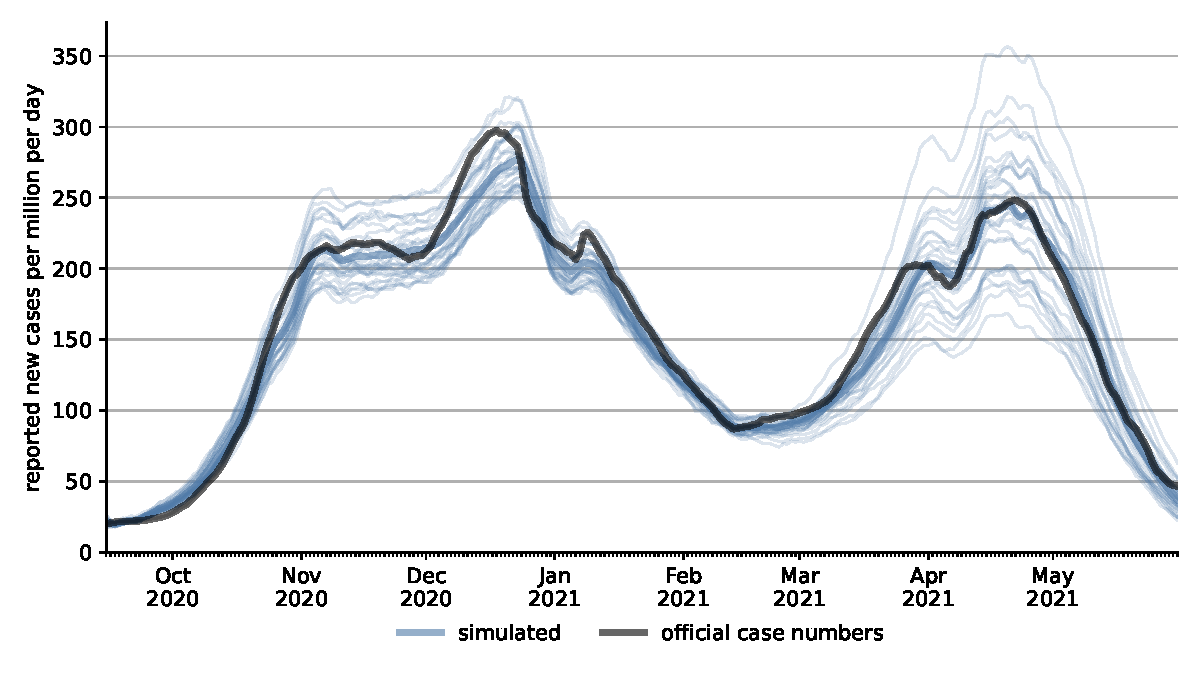
\includegraphics[width=\textwidth]{figures/results/figures/scenario_comparisons/combined_fit/full_new_known_case_with_single_runs}
  \caption{Fit Over the Full Simulation Time Frame with Single Simulation Runs}
  \floatfoot{\noindent \textit{Note:} The figure shows the weekly incidence rates per
  100,000 people for the reported simulated infections rates. The mean infection rate is
  the thick blue line. Single simulation runs are plotted in lighter and thinner lines.
  The official case numbers as reported by the Robert-Koch-Institut are plotted in black.
  The fit is overall very good. The higher the mean incidence and the stronger the growth
  the more variance there is between simulation runs. We averaged over 30 simulation
  runs.}
  \label{fig:aggregated_fit2}
\end{figure}

\begin{figure}[ht]  % newly infected with single runs
  \centering
  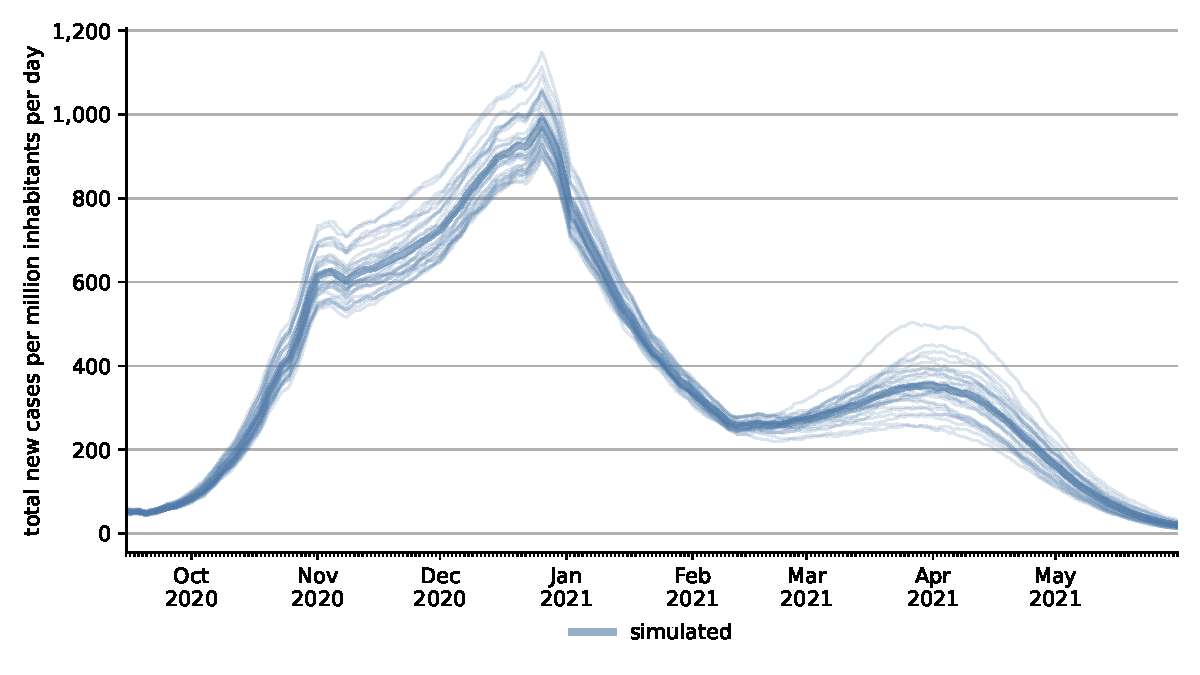
\includegraphics[width=\textwidth]{figures/results/figures/scenario_comparisons/combined_fit/full_newly_infected_with_single_runs}
  \caption{Development of the Total Infections Over the Full Simulation Time Frame with
  Single Simulation Runs}
  \floatfoot{\noindent \textit{Note:} The figure shows the true weekly incidence rates
  per 100,000 people, including undetected cases. The mean infection rate is the thick
  blue line. Single simulation runs are plotted in lighter and thinner lines. The higher
  the mean incidence and the stronger the growth the more variance there is between
  simulation runs. We averaged over 30 simulation runs.}
  \label{fig:newly_infected_in_baseline}
\end{figure}

 \comment[id=K]{More text in this subsection. For \ref{fig:age_group_fit}: Explain why we
 don't fit the 80 to 100 year olds}

\begin{figure}[ht]  % new known case by age group
  \centering
  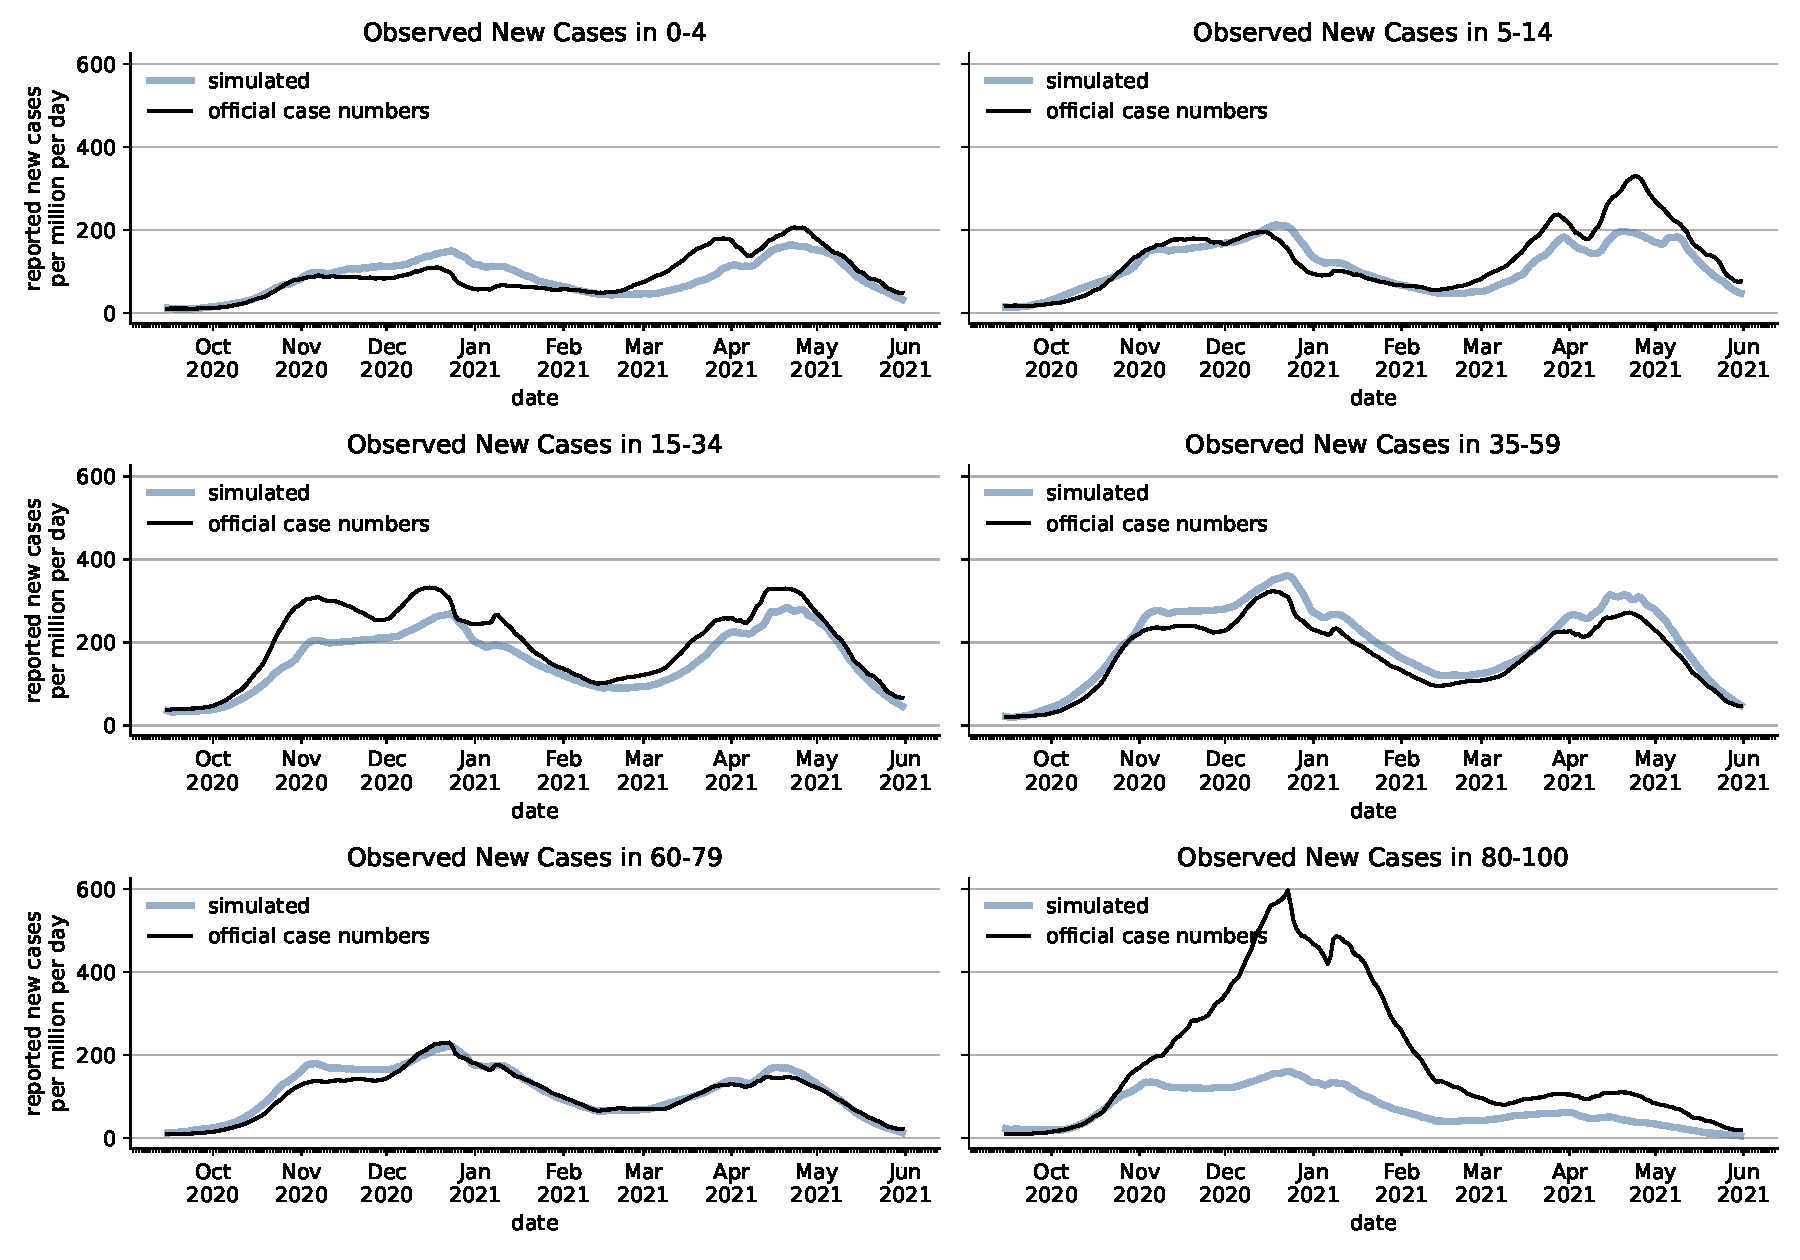
\includegraphics[width=\textwidth]{figures/results/figures/incidences_by_group/age_group_rki/full_combined_baseline_new_known_case}
  \caption{Simulated and Empirical Infections by Age Group}
  \floatfoot{\noindent \textit{Note:} The figure shows the weekly incidence rates per
  100,000 people for the reported versus the simulated infections rates for different age
  groups. The age group of individuals above 80 needs to be interpreted with caution
  because our synthetic population only includes private households, i.e. nursing homes
  are not represented in our model. They accounted for many cases and deaths in the
  winter of 2020 and many 80 to 100 year olds live in these facilities. However, the
  official data does not contain information on whether cases were nursing home
  inhabitants or not. We averaged over 30 simulation runs.}
  \label{fig:age_group_fit}
\end{figure}

 \comment[id=K]{Explain differences between simulated and actual cases in figure
 \ref{fig:state_fit}. (Our states are uniform with respect to their age distribution.}

\begin{figure}[ht]   % new known case by federal state
  \centering
  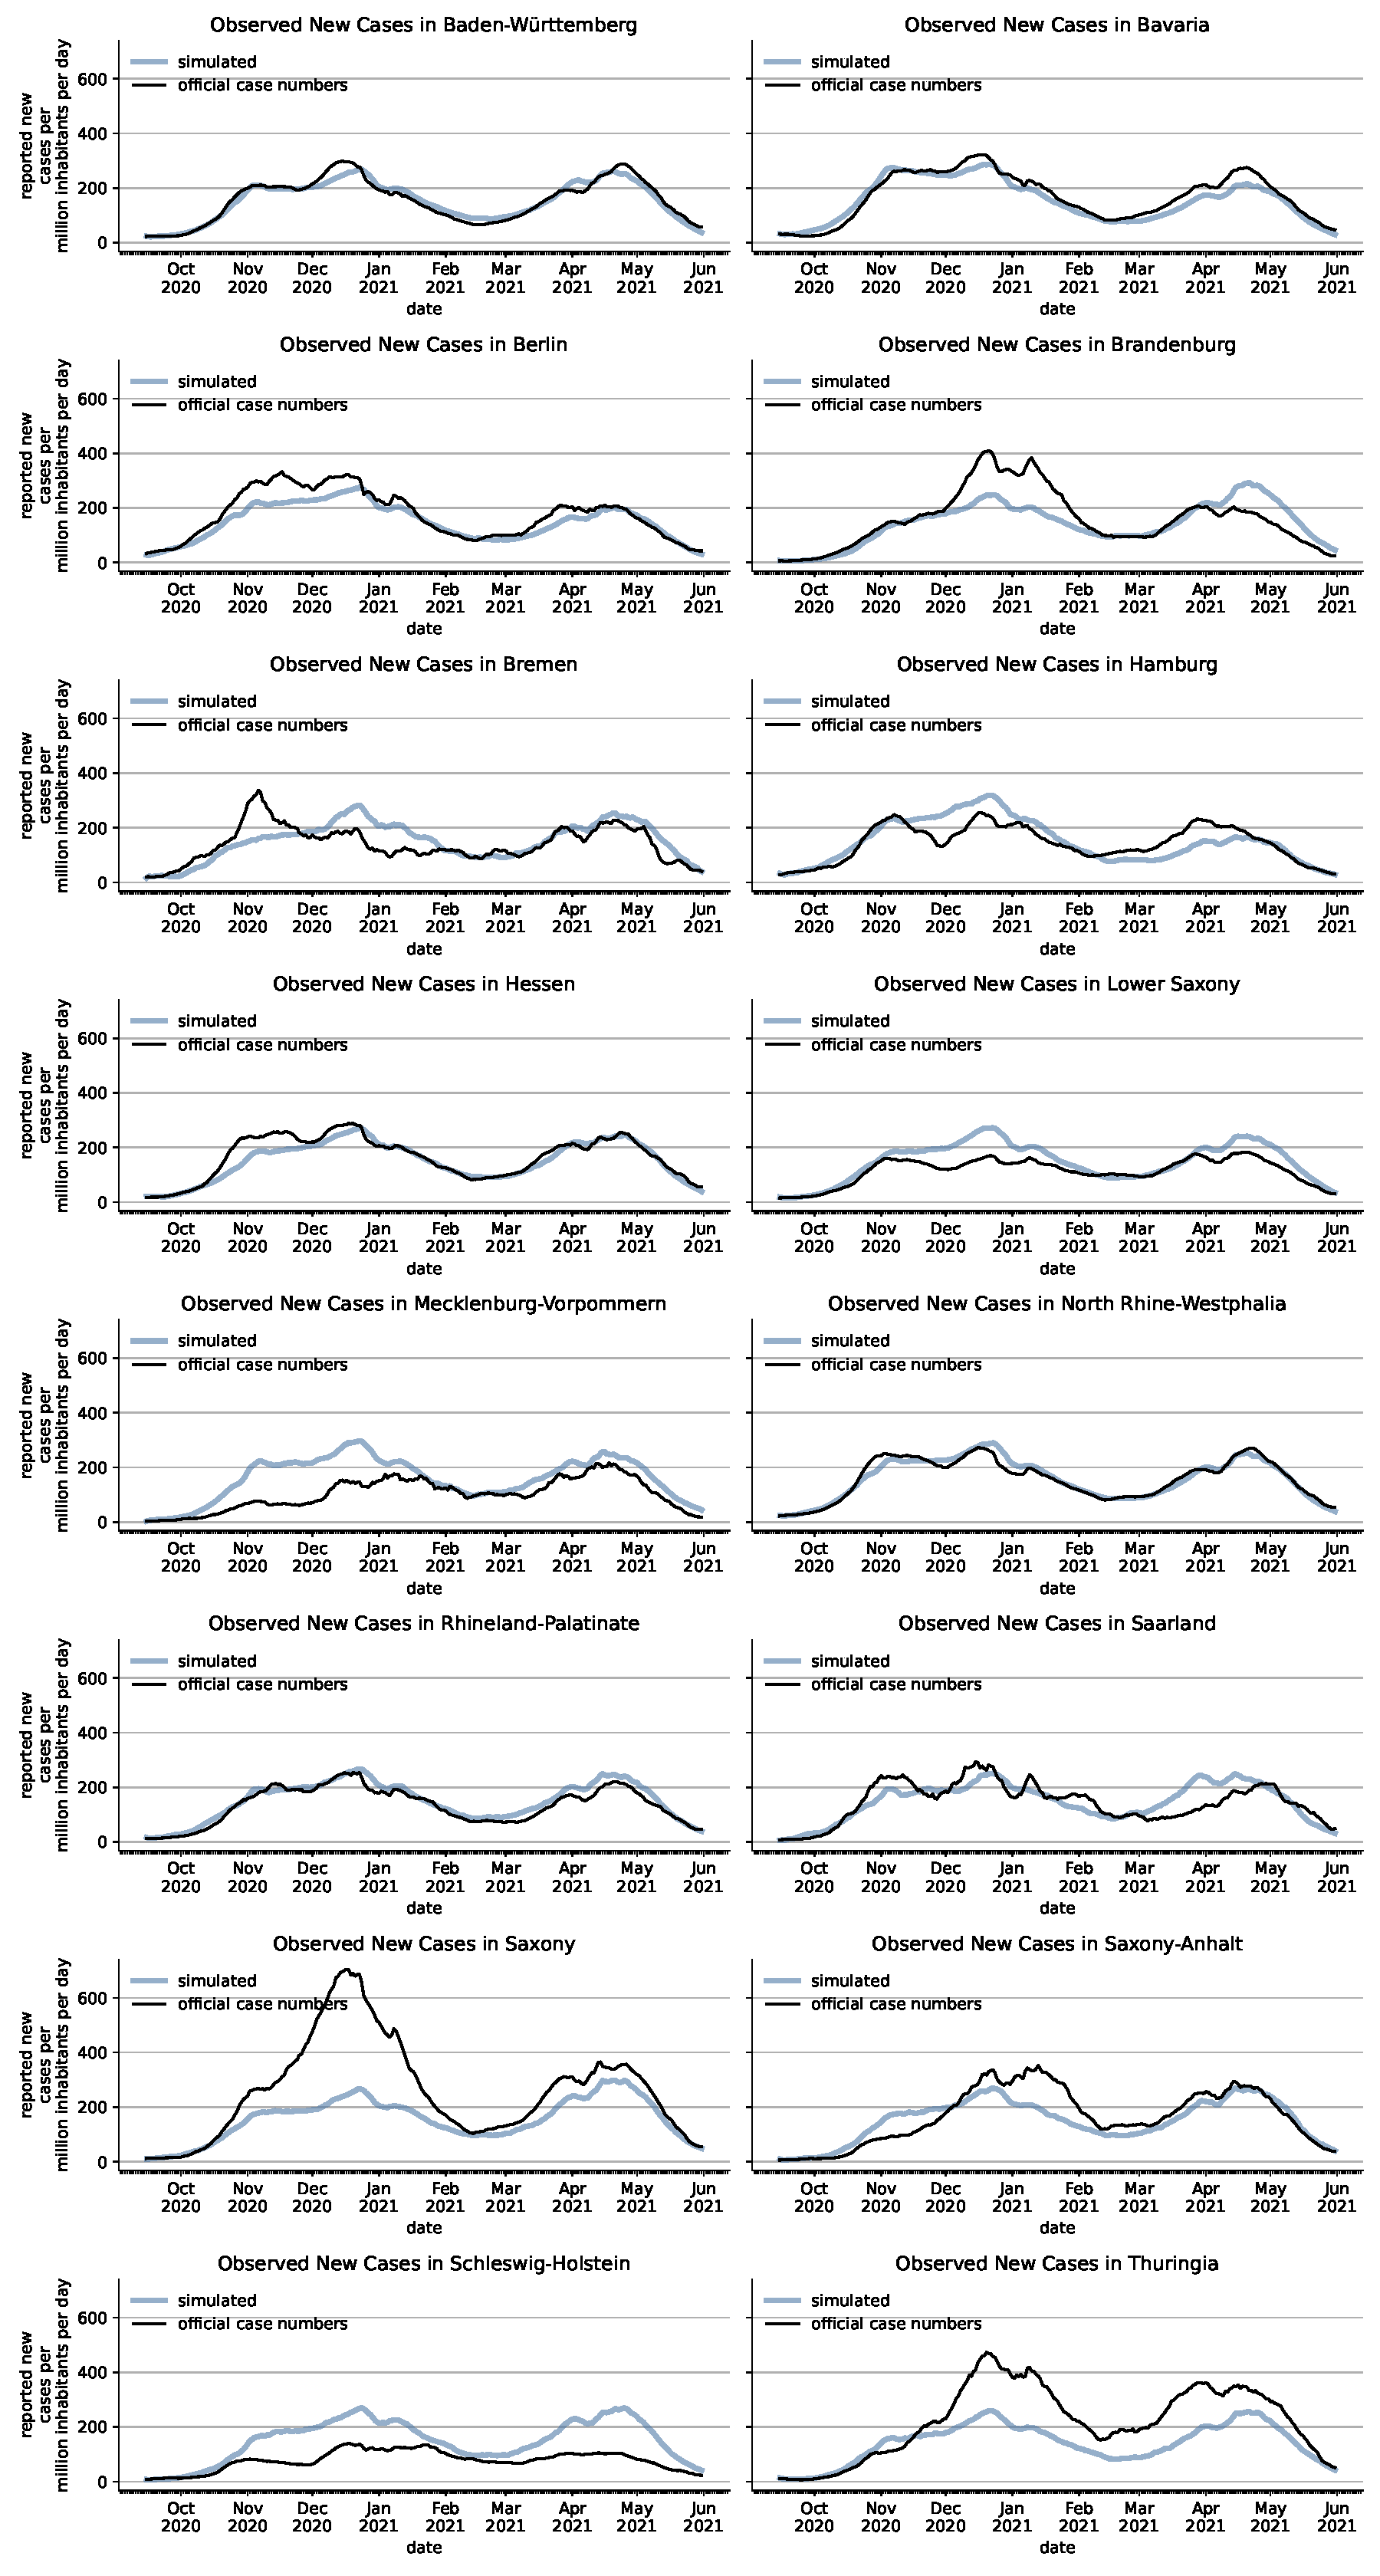
\includegraphics[height=0.95\textheight]{figures/results/figures/incidences_by_group/state/full_combined_baseline_new_known_case}
  \caption{Simulated and Empirical Infections by Federal State}
  \floatfoot{\noindent \textit{Note:} The figure shows the weekly incidence rates per
  100,000 people for the reported versus the simulated infections rates for different
  federal states. We averaged over 30 simulation runs.}
  \label{fig:state_fit}
\end{figure}


\begin{figure}[ht]   % fit of vaccinations
  \centering
  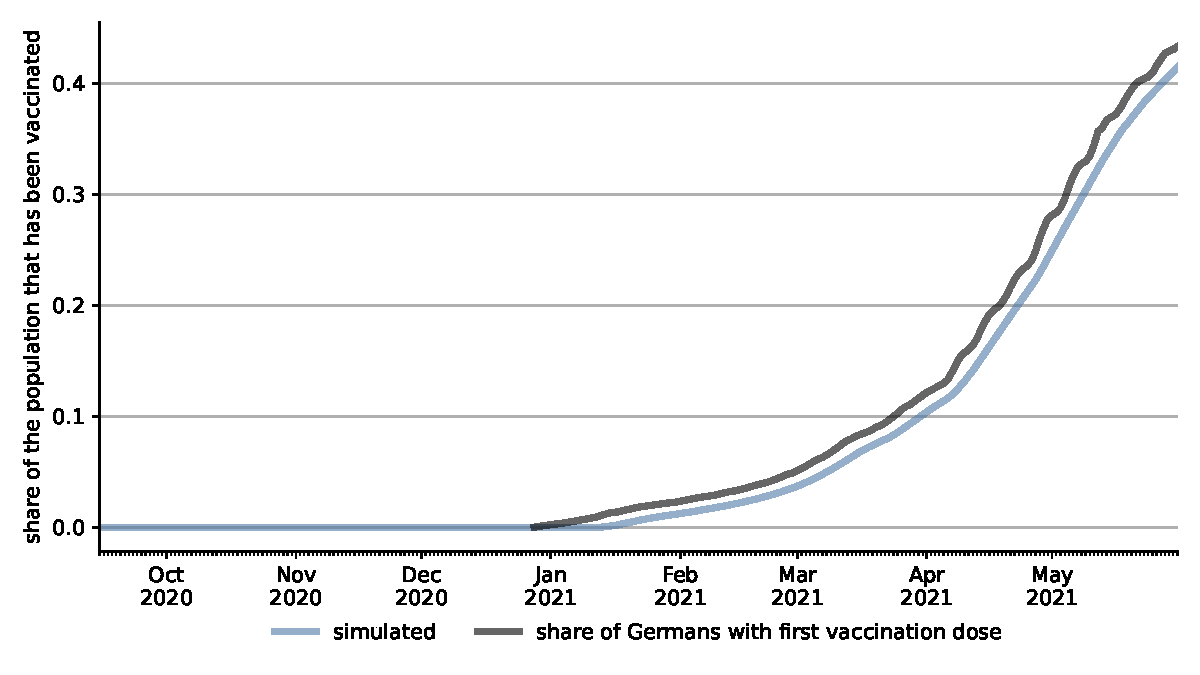
\includegraphics[width=\textwidth]{figures/results/figures/scenario_comparisons/combined_fit/full_ever_vaccinated}
  \caption{Share of Vaccinated Individuals}
  \floatfoot{\noindent \textit{Note:} The figure shows the rate of individuals that are
  vaccinated in our synthetic population versus in the general German population. Note
  that we excluded the vaccinations that were given to nursing homes, approximately the
  first percent of the German population that were vaccinated. Overall, our model covers
  a time frame that goes from zero vaccinated individuals to a state where over 40\% of
  the population are vaccinated. Our vaccinations work imperfectly but we do not model
  different vaccines nor do we distinguish between first and second shot.}
  \label{fig:fit_vaccinations}
\end{figure}


\begin{figure}[ht]   % vaccinations by age group
  \centering
  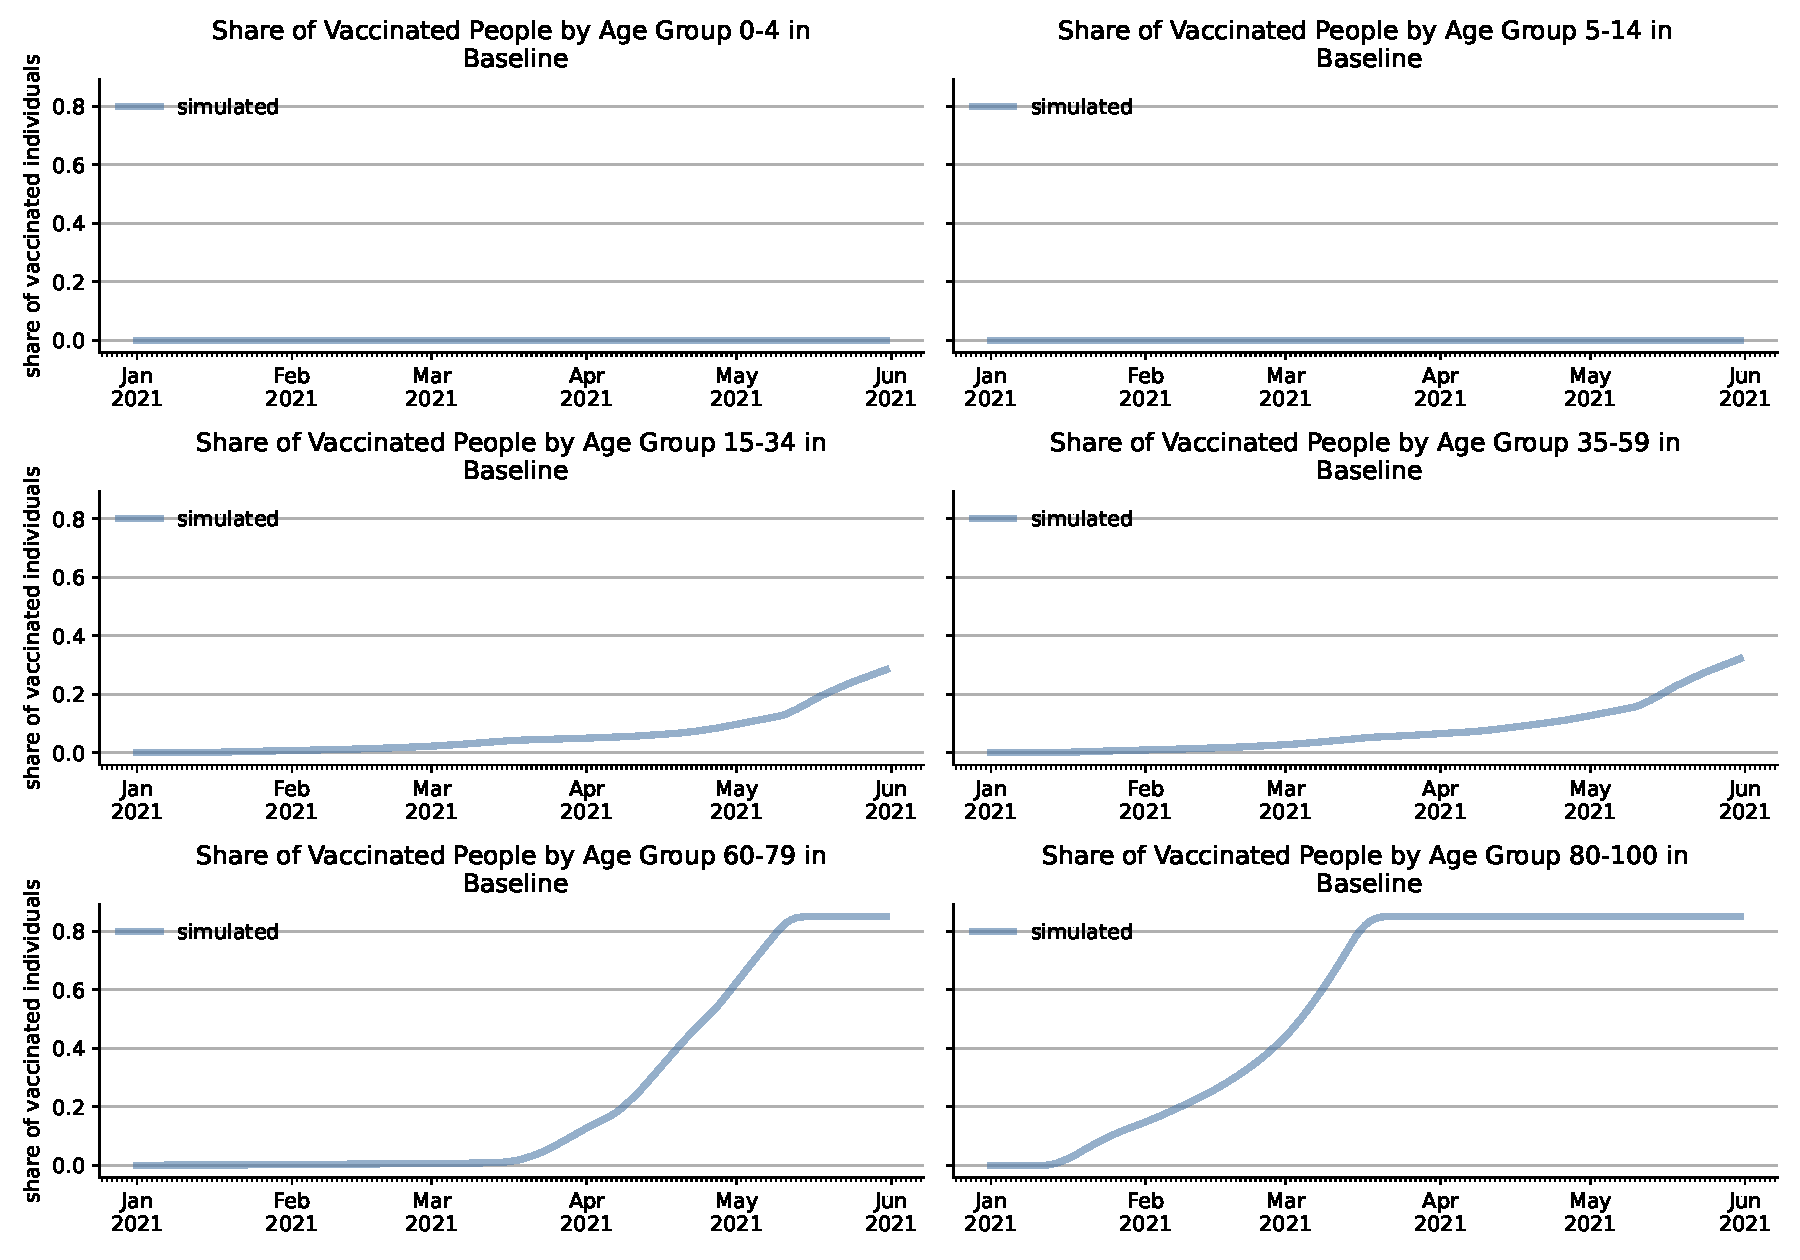
\includegraphics[width=\textwidth]{figures/results/figures/vaccinations/spring_baseline}
  \caption{Simulated and Empirical Infections by Federal State}
  \floatfoot{\noindent \textit{Note:} \textcolor{red}{To be written.}}
  \label{fig:state_fit}
\end{figure}



\begin{figure}[ht]   % R effective
  \centering
  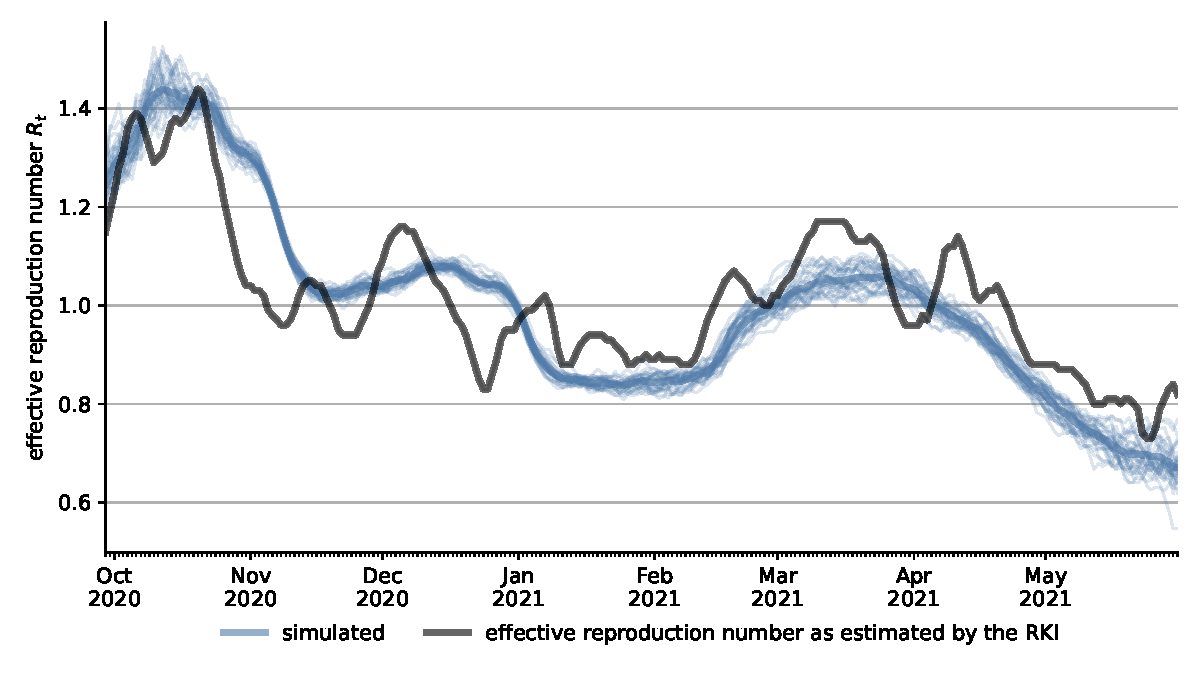
\includegraphics[width=\textwidth]{figures/results/figures/scenario_comparisons/combined_fit/full_r_effective_with_single_runs}
  \caption{Effective Replication Number $R_t$ in the Model and as Reported by the
  Robert-Koch-Institute}
  \floatfoot{\noindent \textit{Note:} The figure shows the effective replication number
  ($R_t$) as reported by the RKI and as calculated in our model. The $R_t$ gives the
  average number of new infections caused by one infected individual. The $R_t$ in our
  model broadly follows the $R_t$ reported by the RKI. Two trends stand out. Firstly, the
  RKI's $R_t$ drops faster in November. This could be due to a change in the testing
  policy that focused tests on the elderly when the second wave hit Germany and led to a
  decline in the overall share of detected cases. The second difference is from mid
  February to mid March where the RKI's reported $R_t$ increased more rapidly than that
  in our model. Here the opposite effect can be expected. During this time rapid tests
  increased strongly leading to more cases being detected. In the short term this leads
  an $R_t$ estimation that is based on detected cases to overestimate the replication
  number.}
  \label{fig:fit_r_effective}
\end{figure}


\begin{figure}[ht]   % Share B.1.1.7
  \centering
  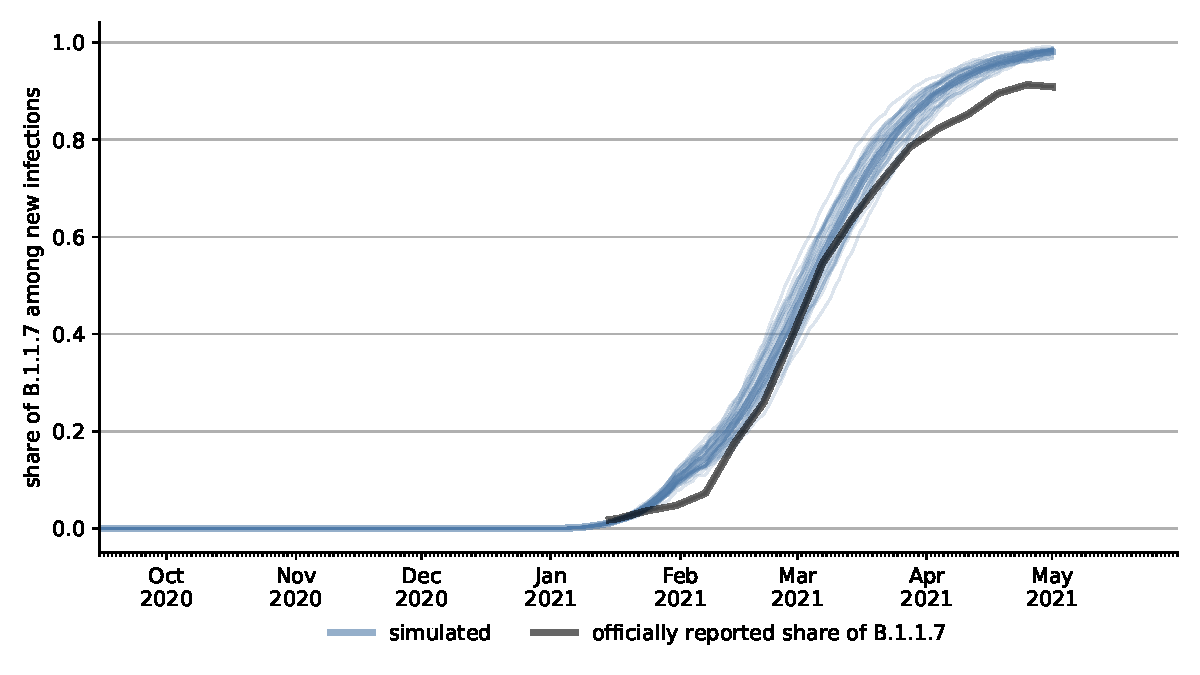
\includegraphics[width=\textwidth]{figures/results/figures/scenario_comparisons/combined_fit/full_share_b117_with_single_runs}
  \caption{Share of B.1.1.7 in the Model and as Reported by the Robert-Koch-Institute}
  \floatfoot{\noindent \textit{Note:} The figure shows the share of B.1.1.7 as
  reported by the RKI and as calculated in our model. We only introduce a few cases over
  the cause of January. From then B.1.1.7 takes over endogenously through its increased
  infectiousness. We model no other features of B.1.1.7. At most we introduce 0.75 cases per 100,000 inhabitants.}
  \label{fig:fit_share_b117}
\end{figure}




\FloatBarrier

